\documentclass{standalone}
\usepackage{tikz}
\usetikzlibrary{patterns, positioning}
\usepackage[sfdefault]{ClearSans} %% option 'sfdefault' activates Clear Sans as the default text font
\usepackage[T1]{fontenc}

\begin{document}
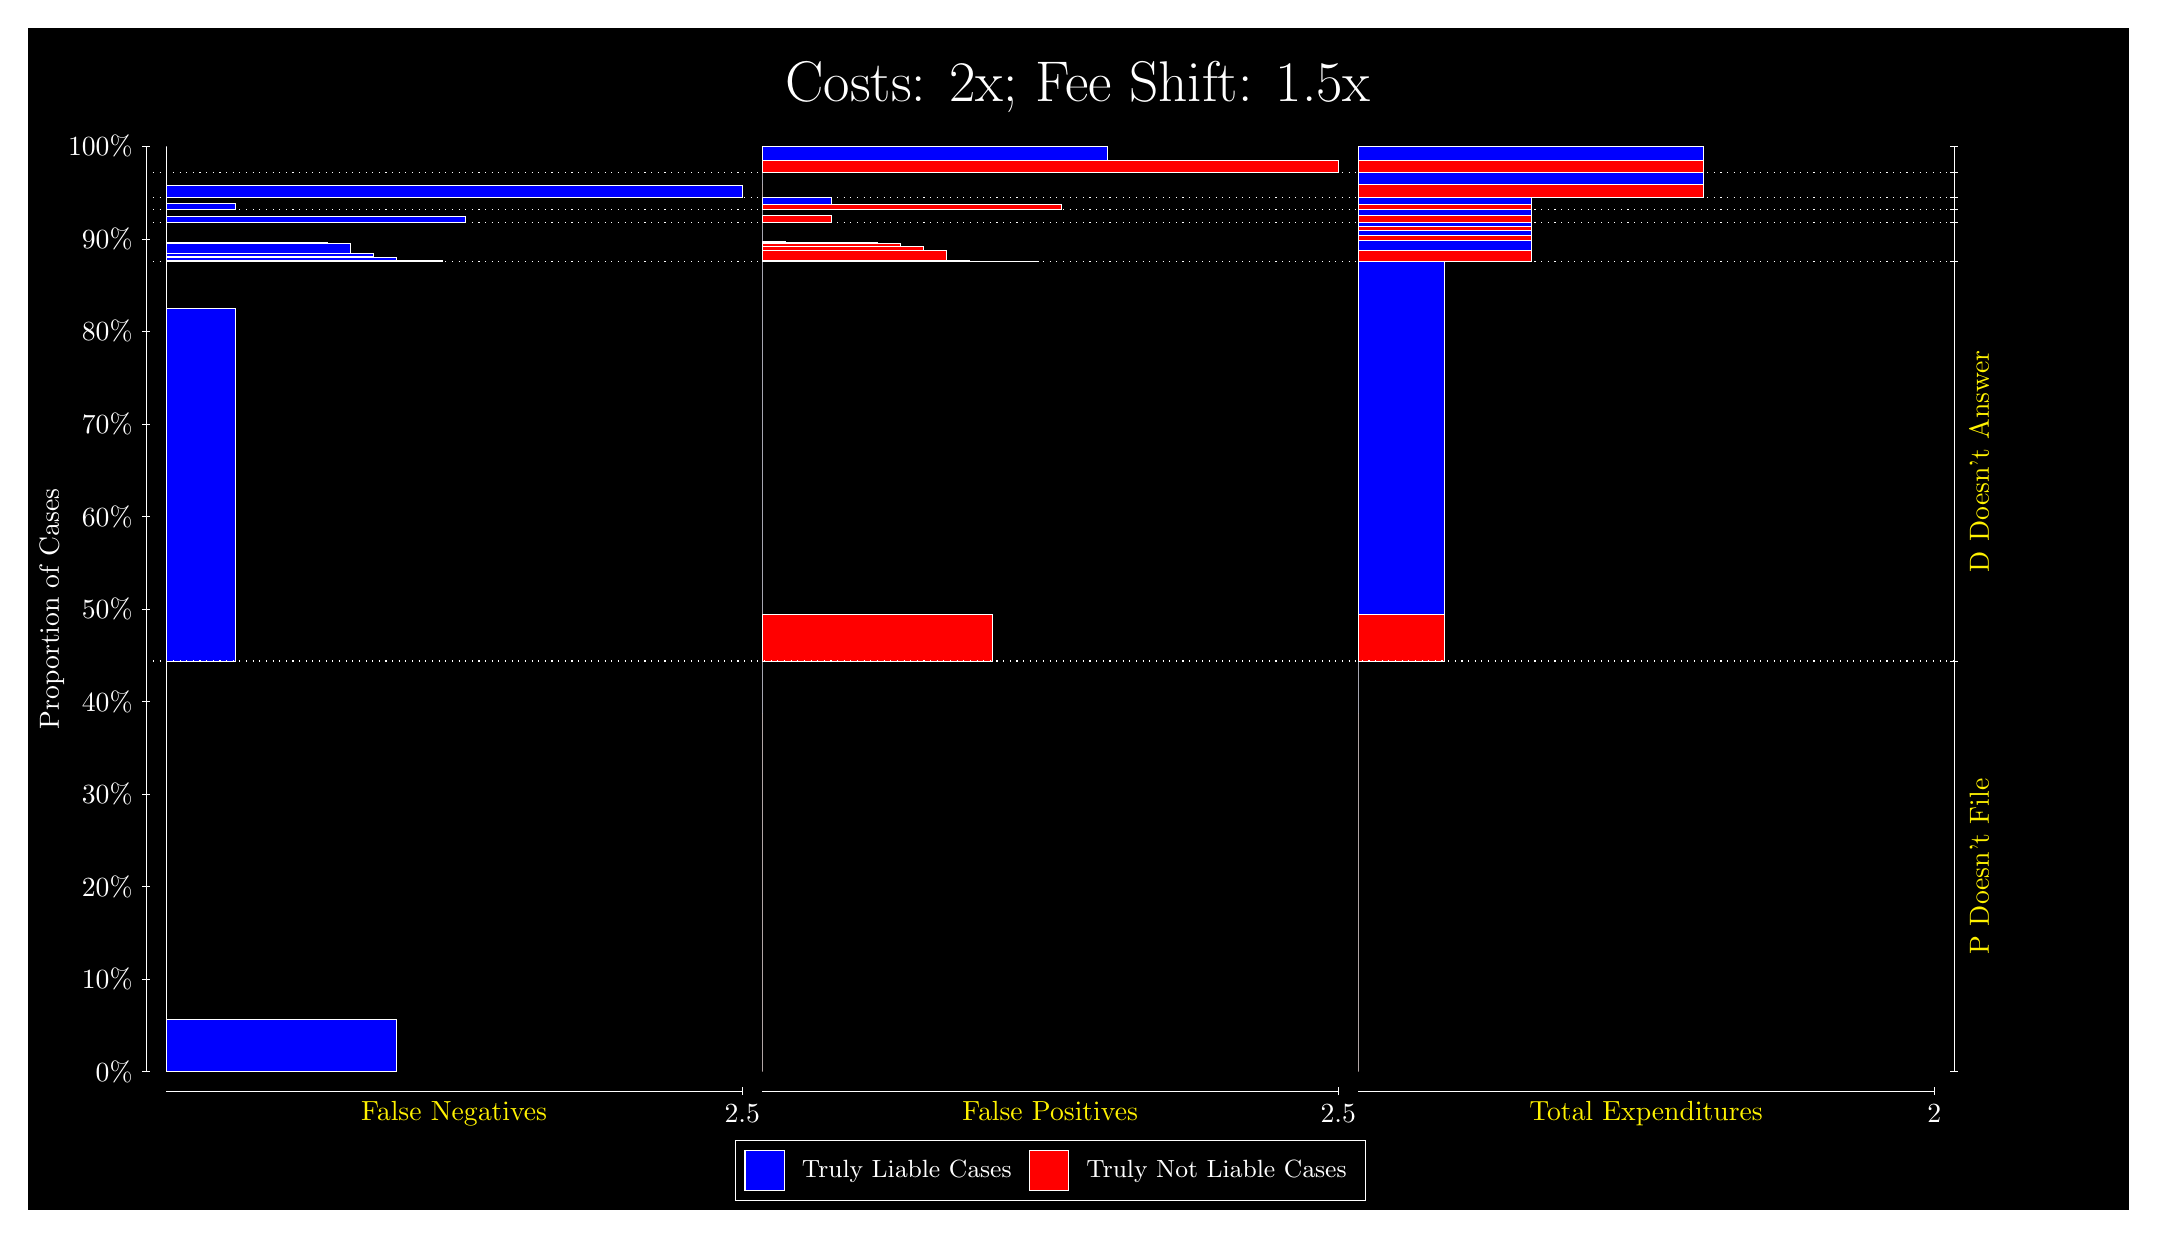
\begin{tikzpicture}
\draw[fill=black] (0,0) rectangle (26.667,15);
\draw[text=white] (0,13.5) rectangle (26.667,15) node[midway] {\huge Costs: 2x; Fee Shift: 1.5x};
\draw[white, very thin] (1.5,1.75) -- (1.5,13.5);
\node[rotate=90, text=white, anchor=center] at (0.3, 7.625) {Proportion of Cases};
\draw[white, very thin] (1.45,1.75) -- (1.55,1.75);
\node[text=white, anchor=east] at (1.45, 1.75) {0\%};
\draw[white, very thin] (1.45,2.925) -- (1.55,2.925);
\node[text=white, anchor=east] at (1.45, 2.925) {10\%};
\draw[white, very thin] (1.45,4.1) -- (1.55,4.1);
\node[text=white, anchor=east] at (1.45, 4.1) {20\%};
\draw[white, very thin] (1.45,5.275) -- (1.55,5.275);
\node[text=white, anchor=east] at (1.45, 5.275) {30\%};
\draw[white, very thin] (1.45,6.45) -- (1.55,6.45);
\node[text=white, anchor=east] at (1.45, 6.45) {40\%};
\draw[white, very thin] (1.45,7.625) -- (1.55,7.625);
\node[text=white, anchor=east] at (1.45, 7.625) {50\%};
\draw[white, very thin] (1.45,8.8) -- (1.55,8.8);
\node[text=white, anchor=east] at (1.45, 8.8) {60\%};
\draw[white, very thin] (1.45,9.975) -- (1.55,9.975);
\node[text=white, anchor=east] at (1.45, 9.975) {70\%};
\draw[white, very thin] (1.45,11.15) -- (1.55,11.15);
\node[text=white, anchor=east] at (1.45, 11.15) {80\%};
\draw[white, very thin] (1.45,12.325) -- (1.55,12.325);
\node[text=white, anchor=east] at (1.45, 12.325) {90\%};
\draw[white, very thin] (1.45,13.5) -- (1.55,13.5);
\node[text=white, anchor=east] at (1.45, 13.5) {100\%};

\draw[white, very thin] (24.457,1.75) -- (24.457,13.5);
\draw[white, very thin] (24.407,1.75) -- (24.507,1.75);
\node[anchor=west] at (24.407, 1.75) {};
\draw[white, very thin] (24.407,6.9643) -- (24.507,6.9643);
\node[anchor=west] at (24.407, 6.9643) {};
\draw[white, very thin] (24.407,12.038) -- (24.507,12.038);
\node[anchor=west] at (24.407, 12.038) {};
\draw[white, very thin] (24.407,12.533) -- (24.507,12.533);
\node[anchor=west] at (24.407, 12.533) {};
\draw[white, very thin] (24.407,12.698) -- (24.507,12.698);
\node[anchor=west] at (24.407, 12.698) {};
\draw[white, very thin] (24.407,12.847) -- (24.507,12.847);
\node[anchor=west] at (24.407, 12.847) {};
\draw[white, very thin] (24.407,13.171) -- (24.507,13.171);
\node[anchor=west] at (24.407, 13.171) {};
\draw[white, very thin] (24.407,13.5) -- (24.507,13.5);
\node[anchor=west] at (24.407, 13.5) {};

\draw[white, very thin, fill=blue] (1.75,1.75) rectangle (4.6775,2.413);
\draw[white, very thin, fill=red] (1.75,2.413) rectangle (1.75,6.9643);
\draw[white, very thin, fill=blue] (1.75,6.9643) rectangle (2.6283,11.445);
\draw[white, very thin, fill=red] (1.75,11.445) rectangle (1.75,12.038);
\draw[white, very thin, fill=blue] (1.75,12.038) rectangle (5.2631,12.047);
\draw[white, very thin, fill=blue] (1.75,12.047) rectangle (4.9703,12.056);
\draw[white, very thin, fill=blue] (1.75,12.056) rectangle (4.6775,12.097);
\draw[white, very thin, fill=blue] (1.75,12.097) rectangle (4.3848,12.098);
\draw[white, very thin, fill=blue] (1.75,12.098) rectangle (4.3848,12.137);
\draw[white, very thin, fill=blue] (1.75,12.137) rectangle (4.092,12.27);
\draw[white, very thin, fill=blue] (1.75,12.27) rectangle (3.7993,12.279);
\draw[white, very thin, fill=blue] (1.75,12.279) rectangle (3.5065,12.283);
\draw[white, very thin, fill=blue] (1.75,12.283) rectangle (3.2138,12.284);
\draw[white, very thin, fill=blue] (1.75,12.284) rectangle (2.921,12.285);
\draw[white, very thin, fill=red] (1.75,12.285) rectangle (1.75,12.533);
\draw[white, very thin, fill=blue] (1.75,12.533) rectangle (5.5558,12.612);
\draw[white, very thin, fill=red] (1.75,12.612) rectangle (1.75,12.698);
\draw[white, very thin, fill=blue] (1.75,12.698) rectangle (2.6283,12.776);
\draw[white, very thin, fill=red] (1.75,12.776) rectangle (1.75,12.847);
\draw[white, very thin, fill=blue] (1.75,12.847) rectangle (9.0689,13);
\draw[white, very thin, fill=red] (1.75,13) rectangle (1.75,13.171);
\draw[white, very thin, fill=red] (1.75,13.171) rectangle (1.75,13.324);
\draw[white, very thin, fill=blue] (1.75,13.324) rectangle (1.75,13.5);
\draw[white, very thin, fill=red] (9.3189,1.75) rectangle (9.3189,6.3013);
\draw[white, very thin, fill=blue] (9.3189,6.3013) rectangle (9.3189,6.9643);
\draw[white, very thin, fill=red] (9.3189,6.9643) rectangle (12.246,7.5579);
\draw[white, very thin, fill=blue] (9.3189,7.5579) rectangle (9.3189,12.038);
\draw[white, very thin, fill=red] (9.3189,12.038) rectangle (12.832,12.039);
\draw[white, very thin, fill=red] (9.3189,12.039) rectangle (12.539,12.04);
\draw[white, very thin, fill=red] (9.3189,12.04) rectangle (12.246,12.044);
\draw[white, very thin, fill=red] (9.3189,12.044) rectangle (11.954,12.054);
\draw[white, very thin, fill=red] (9.3189,12.054) rectangle (11.661,12.186);
\draw[white, very thin, fill=red] (9.3189,12.186) rectangle (11.368,12.226);
\draw[white, very thin, fill=red] (9.3189,12.226) rectangle (11.075,12.267);
\draw[white, very thin, fill=red] (9.3189,12.267) rectangle (10.783,12.276);
\draw[white, very thin, fill=red] (9.3189,12.276) rectangle (10.49,12.286);
\draw[white, very thin, fill=blue] (9.3189,12.286) rectangle (9.9044,12.287);
\draw[white, very thin, fill=blue] (9.3189,12.287) rectangle (9.6116,12.288);
\draw[white, very thin, fill=blue] (9.3189,12.288) rectangle (9.3189,12.533);
\draw[white, very thin, fill=red] (9.3189,12.533) rectangle (10.197,12.619);
\draw[white, very thin, fill=blue] (9.3189,12.619) rectangle (9.3189,12.698);
\draw[white, very thin, fill=red] (9.3189,12.698) rectangle (13.125,12.77);
\draw[white, very thin, fill=blue] (9.3189,12.77) rectangle (10.197,12.847);
\draw[white, very thin, fill=red] (9.3189,12.847) rectangle (9.3189,13.019);
\draw[white, very thin, fill=blue] (9.3189,13.019) rectangle (9.3189,13.171);
\draw[white, very thin, fill=red] (9.3189,13.171) rectangle (16.638,13.324);
\draw[white, very thin, fill=blue] (9.3189,13.324) rectangle (13.71,13.5);
\draw[white, very thin, fill=red] (16.888,1.75) rectangle (16.888,6.3013);
\draw[white, very thin, fill=blue] (16.888,6.3013) rectangle (16.888,6.9643);
\draw[white, very thin, fill=red] (16.888,6.9643) rectangle (17.986,7.5579);
\draw[white, very thin, fill=blue] (16.888,7.5579) rectangle (17.986,12.038);
\draw[white, very thin, fill=red] (16.888,12.038) rectangle (19.083,12.176);
\draw[white, very thin, fill=blue] (16.888,12.176) rectangle (19.083,12.313);
\draw[white, very thin, fill=red] (16.888,12.313) rectangle (19.083,12.374);
\draw[white, very thin, fill=blue] (16.888,12.374) rectangle (19.083,12.434);
\draw[white, very thin, fill=red] (16.888,12.434) rectangle (19.083,12.483);
\draw[white, very thin, fill=blue] (16.888,12.483) rectangle (19.083,12.533);
\draw[white, very thin, fill=red] (16.888,12.533) rectangle (19.083,12.619);
\draw[white, very thin, fill=blue] (16.888,12.619) rectangle (19.083,12.698);
\draw[white, very thin, fill=red] (16.888,12.698) rectangle (19.083,12.77);
\draw[white, very thin, fill=blue] (16.888,12.77) rectangle (19.083,12.847);
\draw[white, very thin, fill=red] (16.888,12.847) rectangle (21.279,13.019);
\draw[white, very thin, fill=blue] (16.888,13.019) rectangle (21.279,13.171);
\draw[white, very thin, fill=red] (16.888,13.171) rectangle (21.279,13.324);
\draw[white, very thin, fill=blue] (16.888,13.324) rectangle (21.279,13.5);
\draw[white, dotted] (1.5,6.9643) -- (24.457,6.9643);
\draw[white, dotted] (1.5,12.038) -- (24.457,12.038);
\draw[white, dotted] (1.5,12.533) -- (24.457,12.533);
\draw[white, dotted] (1.5,12.698) -- (24.457,12.698);
\draw[white, dotted] (1.5,12.847) -- (24.457,12.847);
\draw[white, dotted] (1.5,13.171) -- (24.457,13.171);
\draw[white, very thin] (1.75,1.5) -- (9.0689,1.5);
\node[text=yellow, anchor=north] at (5.4094, 1.5) {False Negatives};
\draw[white, very thin] (9.0689,1.45) -- (9.0689,1.55);
\node[text=white, anchor=north] at (9.0689, 1.45) {2.5};

\draw[white, very thin] (9.3189,1.5) -- (16.638,1.5);
\node[text=yellow, anchor=north] at (12.978, 1.5) {False Positives};
\draw[white, very thin] (16.638,1.45) -- (16.638,1.55);
\node[text=white, anchor=north] at (16.638, 1.45) {2.5};

\draw[white, very thin] (16.888,1.5) -- (24.207,1.5);
\node[text=yellow, anchor=north] at (20.547, 1.5) {Total Expenditures};
\draw[white, very thin] (24.207,1.45) -- (24.207,1.55);
\node[text=white, anchor=north] at (24.207, 1.45) {2};

\node[text=yellow, centered, rotate=90] at (24.777, 4.3571) {P Doesn't File};
\node[text=yellow, centered, rotate=90] at (24.777, 9.5014) {D Doesn't Answer};






\draw (12.978300999999998,1.5) node[draw=none] (baseCoordinate) {};
\begin{scope}[align=center]
        \matrix[scale=0.5, draw=white, below=0.5cm of baseCoordinate, nodes={draw}, column sep=0.1cm]{
            \node[rectangle, draw, minimum width=0.5cm, minimum height=0.5cm, fill=blue] {}; &
            \node[draw=none, font=\small, text=white] (B) {Truly Liable Cases}; &
            \node[rectangle, draw, minimum width=0.5cm, minimum height=0.5cm, fill=red] {}; &
            \node[draw=none, font=\small, text=white] (B) {Truly Not Liable Cases}; \\
            };
\end{scope}

\end{tikzpicture}
\end{document}